\documentclass[tikz]{standalone}
% To convert from pdf to png use the following :
%
% C:\cygwin64\bin\convert.exe -density 600 overlay.pdf -size 240x240 overlay.png
%

\usepackage{listings}
\usepackage{luatex85}

\usetikzlibrary{positioning}
\usetikzlibrary{calc}
\usetikzlibrary{backgrounds}
\usetikzlibrary{decorations.text}

\begin{document}
%
% Importer : Encased
%
% This traps the import at multiple entry points representing 
% the most complete importer one may produce.
%

% Anti-spokes
%
% The idea is to draw an anti-spoke or paddles with this diagram.
%
% \begin{tikzpicture}
% \draw let \n{spokes}={3}, \n{arc}={360/\n{spokes}}, \n{angoff}={-\n{arc}+30} in foreach[evaluate = \idx as \ray using \idx/\n{spokes}*360] \idx in {1,2,...,\n{spokes}}
%  {(0,0) -- (\ray+\n{angoff}:1em) (\ray+\n{angoff}+\n{arc}/2:2em) -- (\ray+\n{angoff}-\n{arc}/2:2em)};
% \end{tikzpicture}
%
%
% \begin{tikzpicture}
% \draw [rounded corners]
%   let \n{spokes}={3}, 
%       \n{arc}={360/\n{spokes}}, \n{angoff}={-\n{arc}+30}, 
%       \n{Radius}={6em}, \n{radius}={1em} 
%   in foreach[evaluate = \idx as \ray using \idx/\n{spokes}*360] \idx in {1,2,...,\n{spokes}}
%  {(\ray+\n{angoff}:\n{radius}) -- (\ray+\n{angoff}+\n{arc}/2:\n{Radius}) -- (\ray+\n{angoff}-\n{arc}/2:\n{Radius}) -- cycle};
% \end{tikzpicture}

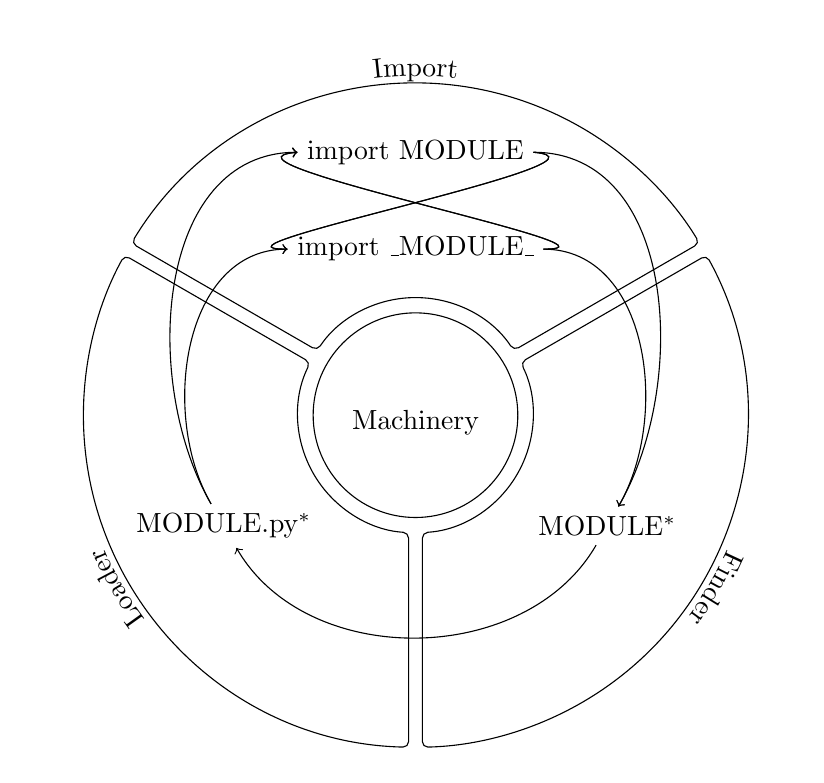
\begin{tikzpicture}[
 arc label/.style={
  decorate,
  decoration={ 
   text along path,
   text align=center,
   reverse path=true,
   text={#1}
   }}]
\coordinate (ctr) {}; % Used as an anchor for later nodes
% Mechanism Componenets
\foreach 
  [var=\spokes,  evaluate=\spokes using    3,
   var=\radius,  evaluate=\radius using 4.25,% 3.25, 
   var=\Radius,  evaluate=\Radius using   12, 
   var=\width,   evaluate=\width  using 0.25, 
   var=\offset,  evaluate=\offset using 0.25, 
   var=\arc,     evaluate=\arc    using 360/\spokes,
   var=\inner,   evaluate=\inner  using {\arc/2-2*asin(\width/2/\radius)},
   var=\outer,   evaluate=\outer  using {\arc/2-2*asin(\width/2/\Radius)},
   var=\rotate,  evaluate=\rotate using \arc/2+30,
   count=\count from 0, evaluate = \idx as \ray using \count/\spokes*360] \text in {Import, Loader, Finder} 
  {\draw [rounded corners = 0.2em]
     (\ray+\rotate-\inner:\radius em) arc(\ray+\rotate-\inner:\ray+\rotate+\inner:\radius em) -- 
     (\ray+\rotate+\outer:\Radius em) arc(\ray+\rotate+\outer:\ray+\rotate-\outer:\Radius em) -- cycle;
   \draw[arc label = \text] let \n{radius} = {\offset+\Radius} in (\rotate+\ray-\outer:\n{radius} em) arc (\rotate+\ray-\outer:\rotate+\ray+\outer:\n{radius} em);};
% \node (int) at (ctr)                 [draw, fill=black, text=white, circle, inner sep = 1em] {Machinery};
% Overlay Mechanism
\node[align=center] (imp) at ($(ctr) + ( 90:   6em)$) {\lstinline[]|import _MODULE_|};
\node[align=center] (fdr) at ($(ctr) + (-30:   8em)$) {\lstinline[]|MODULE|$^{*}$};
\node[align=center] (ldr) at ($(ctr) + (210:   8em)$) {\lstinline[]|MODULE.py|$^{*}$};
\node[align=center] (Imp) at ($(ctr) + ( 90: 9.5em)$) {\lstinline[]|import MODULE|};
% \node (int) at (ctr)                 [draw, circle, align=center] {\\ Machinery};
\node (int) at (ctr)                 [draw, circle, inner sep = 1em, align=center] {\\ Machinery};
%% Looping Structure
% Internal Structure
% \draw[->, shorten >=0.5em, shorten <=0.5em, gray, dashed]  (int.60) to [out = 240, in = 180]   (int.0);
% \draw[->, shorten >=0.5em, shorten <=0.5em, gray, dashed] (int.180) to [out =   0, in = -60] (int.120);
% \draw[->, shorten >=0.5em, shorten <=0.5em, gray, dashed] (int.300) to [out = 120, in =  60] (int.240);
% External Structure   
% \draw[->] (int) to [in =  60, out =   0] (fdr);
% \draw[->] (fdr) to [in = 300, out = 240] (int);
% \draw[->] (int) to [in = 300, out = 240] (ldr);
% \draw[->] (ldr) to [in = 180, out = 120] (int);
% Primary Import
% \draw[->] (int.120) .. controls ++(120:1em) and ++(180:2em) .. (imp.180);
% \draw[->]   (imp.0) .. controls ++(  0:2em) and ++( 60:1em) .. (int.60);
% Secondary Import
% \draw[->] (int.120) .. controls ++(150:  1em) and ++(185:8.5em) .. (Imp.180);
% \draw[->]   (Imp.0) .. controls ++( -5:8.5em) and ++( 60:  1em) .. (int.60);
% Switching
\draw[->] (Imp.0) to[out =  -5, in = 180] (imp);
\draw[->]   (imp) to[out =   0, in = 185] (Imp.180);
%% Swooping Structure
% Structure
\draw[->] (imp) to[out =   0, in =  60] (fdr);
\draw[->] (fdr) to[out = 240, in = 300] (ldr);
\draw[->] (ldr) to[out = 120, in = 180] (imp);
\draw[->] (Imp) to[out =   0, in =  60] (fdr);
\draw[->] (ldr) to[out = 120, in = 180] (Imp);
% Switching
\draw[->] (Imp.0) to[out =  -5, in = 180] (imp);
\draw[->]   (imp) to[out =   0, in = 185] (Imp.180);
\end{tikzpicture}

\end{document}